% Compile twice: pdflatex -interaction=nonstopmode -halt-on-error main.tex
\documentclass[10pt,a4paper,twocolumn]{article}
\usepackage[left=18mm,right=18mm,top=17mm,bottom=17mm,columnsep=6mm]{geometry}
\usepackage[T1]{fontenc}
\usepackage[utf8]{inputenc}
\usepackage{mathptmx}
\usepackage{amsmath,amssymb,graphicx,booktabs,array,tabularx,longtable}
\usepackage{microtype}
\usepackage{titlesec}
\titleformat{\section}{\large\bfseries}{\thesection}{0.6em}{}
\titleformat{\subsection}{\normalsize\bfseries}{\thesubsection}{0.6em}{}
\titlespacing*{\section}{0pt}{9pt plus 2pt minus 1pt}{4pt}
\titlespacing*{\subsection}{0pt}{7pt plus 2pt minus 1pt}{3pt}
\usepackage[font=small,labelfont=bf]{caption}
\usepackage{xcolor}
\usepackage{xurl}
\usepackage[colorlinks=true,allcolors=blue!45!black]{hyperref}
\urlstyle{same}
\hypersetup{pdftitle={Multi-Horizon Forecasting of Apple Stock Prices and Returns Across Temporal Scales},pdfauthor={Wang Yang}}
\usepackage{flushend}
\providecommand{\tightlist}{\setlength{\itemsep}{0pt}\setlength{\parskip}{0pt}}
\setlength{\parindent}{1em}
\setlength{\parskip}{0pt}
\raggedbottom
\setlength{\textfloatsep}{10pt plus 2pt minus 2pt}
\setlength{\floatsep}{8pt plus 2pt minus 2pt}
\setlength{\intextsep}{9pt plus 2pt minus 2pt}
\setcounter{topnumber}{3}
\setcounter{totalnumber}{5}
\renewcommand{\topfraction}{0.9}
\renewcommand{\textfraction}{0.08}
\newcommand{\emailaddress}{[Email to be completed by the author]}
\title{\bfseries Multi-Horizon Forecasting of Apple Stock Prices and Returns Across Temporal Scales}
\author{Wang Yang\\High School Affiliated to Shanghai Jiao Tong University\\Shanghai 200439, China\\\small\emailaddress}
\date{}
\begin{document}
\maketitle
\section*{Abstract}
Neural forecasts of stock prices can improve substantially after a change in initialization and still offer little advantage over the current price. We examine this discrepancy in AAPL price and cumulative-return forecasts across five temporal scales and twenty tasks. An eight-method comparison is followed by matched interventions on the forecast's initial function, price anchor and training cap. Zero-return initialization reduces xPatch error by 9.60\% at minute H60 and 44.11\% at hourly H8 relative to its default implementation. After calibration, both remain slightly worse than zero. On hourly prices, extending default training from twenty to sixty epochs leaves much larger errors than initializing at the current price. Annual forecasts improve over persistence and zero, but their advantage over a shrunk unconditional mean is unresolved. A separate reference using Apple's announced 2020 split reduces monthly price and return errors by 76.81\% and 73.60\%, changing the model comparison without changing any prediction. These results identify implementation and reference-information effects that would be obscured by architecture rankings alone. They come from development-exposed history; a new method with stable gains over strong controls remains to be established.

\noindent\textbf{Keywords:} stock forecasting; multiple horizons; initialization; forecast calibration; corporate actions.

\section{Introduction}\label{sec:introduction}

A model that predicts tomorrow's stock price has today's price available. Reproducing that level should be easy, yet a directly trained neural network may spend much of a short training run learning to do so. A poor result can then reflect the starting function and optimization budget as well as the difficulty of forecasting the price change. Conversely, a large reduction in neural-network error may merely bring the forecast back toward persistence. This distinction matters when interpreting improvements between models.

Our AAPL experiments began with a comparison across annual, quarterly, monthly, hourly and minute scales. Large errors in some default networks prompted a closer question: which part of the result is attributable to the implemented forecasting procedure, and which part survives a stronger reference? We retain all twenty price/return tasks, then examine particular contrasts through matched changes to initialization and the nominal-price anchor. The purpose is to explain observed differences before treating them as evidence for a better architecture.

The architecture literature supplies useful forecasting components. xPatch separates seasonal and trend streams after exponential decomposition \cite{r1}; PatchTST uses patching and channel independence \cite{r2}; Temporal Fusion Transformers address interpretable multi-horizon prediction \cite{r3}. General convolutional/recurrent comparisons also motivate testing more than one sequence model \cite{r13}. Their results do not determine whether an AAPL forecast will beat persistence under the targets and training budget used here.

Financial applications differ in their targets and information. Reviews cover a broad range of stock-market inputs and evaluation choices \cite{r4}. DeepLOB uses limit-order-book information \cite{r5}, while other work studies multi-horizon intraday returns \cite{r6} and financial foundation models \cite{r7}. Kamalov et al.~compare prices and returns as \emph{inputs} to directional classifiers \cite{r8}; here prices and cumulative returns are separately fitted \emph{targets}. Mattera et al.~already include AAPL in multi-horizon stock-price forecasting with clustering and reconciliation \cite{r9}. We do not compare directly with their reconciliation procedure.

Forecast combinations and expert mixtures have a long history \cite{r14,r15}, and historical averages are demanding return-forecasting controls \cite{r16}. Likewise, zero-head initialization, residual targets and scalar shrinkage are familiar constructions. The evidence offered here is the controlled comparison of these choices in a particular forecasting study. Its clearest finding is that correcting a weak initial function can account for much of an apparent model gain. The long-scale results then show why the remaining gain needs a different assessment: unconditional forecasts, overlapping outcomes and a known stock split change its interpretation.

\section{Data and temporal evaluation}\label{sec:data}

\subsection{Prices, returns and trading clocks}

The reported experiments use Alpaca SIP/raw observations before July 1, 2026, New York time. The author reports research permission from Alpaca and Kibot; Kibot data are not used in these results. The daily source contains 2,637 rows from January 2016 through June 2026. Conservative completion retains 2,636 dates and 125 complete months. Intraday data cover January 4, 2021--June 30, 2026, with 535,620 expected regular-session minutes and 8,238 complete hourly bars on the XNYS grid. Minute-derived closes need not equal official closing-auction prices.

At a completed origin \(t\), the two targets are
\[
Y^P_{t,j}=P_{t+j},\qquad
Y^R_{t,j}=\log(P_{t+j}/P_t),\quad j=1,\ldots,H.
\]
Table~\ref{tab:design} gives the ten horizons; fitting both targets gives twenty tasks. A horizon counts retained trading bars. Hourly H8 can cross a session boundary and includes the intervening overnight change; it is not eight clock hours. Incomplete hourly remnants are excluded, whereas minute paths must finish in the same regular session.

\begin{table}[t]
\centering\small
\caption{Task definitions. Lookback and horizon are measured in the bar units of the second column.}\label{tab:design}
\setlength{\tabcolsep}{4pt}
\begin{tabular}{llrr}\toprule
Scale & Bar & Lookback & Horizon \(H\)\\\midrule
Annual & Month & 12 & 12\\
Quarterly & Month & 36 & 3\\
Monthly & Day & 252 & 21\\
Hourly & Complete hour & 96 & 1, 4, 8\\
Minute & Regular minute & 480 & 5, 15, 30, 60\\\bottomrule
\end{tabular}
\end{table}

Historical input windows adjust only for splits effective by the origin. Future nominal-price targets retain later split discontinuities; dividends are excluded. This definition matters for the monthly result in Section~\ref{sec:split}. Daily bars become available conservatively at the next New York midnight, consistent with the aggregation convention \cite{r12}. This rule specifies the assumed decision time rather than establishing the point-in-time status of subsequently revised vendor data.

\subsection{Splits, losses and uncertainty}

Five expanding folds separate fitting, inner stopping and calibration, and outer assessment. Each boundary removes earlier origins whose labels are not yet complete. Formally, if \(\ell(t,H)\) is the completion time of the last target bar and \(\tau_{\rm next}\) the next partition's first decision time, origins with \(\ell(t,H)\geq\tau_{\rm next}\) are purged. Scalers are estimated on the inner fit only. The inner stopping tail controls both early stopping and the scalar calibration described below.

The eight methods are persistence, drift, seasonal repetition, Ridge, MLP, GRU, LSTM and adapted xPatch. The original neural comparison comprises 400 fits. Neural training uses Adam, learning rate 0.001, batches of 128, patience three and a twenty-epoch cap. The primary score is endpoint MSE; the archive also retains endpoint MAE and path error. Price persistence predicts the current close and the return reference predicts zero. For either target,
\[
I=100\left(1-\frac{\operatorname{MSE}_{\rm model}}
                         {\operatorname{MSE}_{\rm reference}}\right)\%.
\]
Positive values indicate lower error than the named reference. Price and return losses are never pooled together.

When several seeds are available, losses are averaged at each origin before pooling:
\[
L_t=\frac{1}{S}\sum_{s=1}^{S}(y_t-\hat y_{t,s})^2.
\]
This evaluates a training procedure over seeds. Scoring the mean prediction instead would evaluate an ensemble and generally produce a different MSE.

Paired moving-block intervals use 5,000 draws and seed 2026 \cite{r10,r11}. Blocks span one/five sessions for minute tasks and two/five sessions for hourly tasks. Annual and quarterly blocks contain 12/24 and 3/6 monthly groups; monthly tasks use 21/42 daily groups. Intraday folds remain separate strata. Long-scale chronological groups concatenate because an annual fold can be shorter than a block. We report both block lengths. The intervals are nominal historical summaries, without adjustment for repeated screening; the implications of development exposure are considered in Section~\ref{sec:discussion}.

\section{Matched interventions}\label{sec:methods}

\subsection{Changing the initial function}

The initial audit found several differences between the original networks and an earlier small model: the latter omitted the nominal-price anchor, began at a baseline forecast, used residual price outputs and could stop relative to its epoch-zero loss. Those differences made its apparently better behavior ambiguous. We therefore changed them separately in the original implementations.

For returns, a four-cell design crosses default versus exact-zero-return initialization with an observed versus constant-zero standardized nominal-price anchor. Architectures, past log-relative histories, seeds, path loss and training rules are matched. Removing the anchor therefore tests a particular input route rather than removing price history altogether. The hourly-H1 price diagnostic separately crosses direct-price versus dollar-residual outputs with default versus current-price-function initialization. Each representation has its own fit-only target scaler, so this latter contrast combines representation and scaling.

The first two chronological folds and seed 2026 screen the specified contrasts. A contrast must improve in both folds before its complete four-cell design is repeated over five folds and seeds 2026--2028. This admits xPatch minute-H60/hourly-H8 returns and LSTM/xPatch hourly-H1 prices. The replication comprises 240 cells, including reused screening cells. The LSTM return and small-model stopping branches do not pass. Restored default weights and stopping epochs match their archived counterparts exactly, supporting the comparison with the original procedure.

Zero initialization has an optimization consequence as well as an output consequence. For a head \(f=Wg_\theta+c\), setting \(W=0\) removes the first loss gradient through \(g_\theta\). All 120 replicated baseline-initialized cells show this zero first backbone gradient, with learned gradients thereafter. Thus the experiment changes both the starting forecast and the first updates; it cannot attribute the entire effect to the starting output alone.

\subsection{Longer training and post-training shrinkage}

To test whether the poor default merely needs more training, thirty hourly-H1 price fits continue from their twenty-epoch checkpoints with a sixty-epoch cap. Optimizer state, random state, batch position and the original early-stop rule are retained. Seventeen fits had reached the original cap; the other thirteen receive no additional updates. This comparison preserves the training trajectory rather than introducing a fresh random restart.

We then apply one xPatch recipe to all twenty tasks. Architecture precedence and the hourly-H1 initialization criterion were specified before reading the full replication summary. The selected recipe retains the original observed-anchor inputs, direct targets and path loss, but begins at zero returns or the current price. Its trained departure \(q=f-b\) from the baseline \(b\) is calibrated on inner-stop endpoints:
\[
\hat y=b+\alpha(f-b),\qquad
\alpha=\operatorname{clip}_{[0,1]}
             \left(\frac{\sum q(y-b)}{\sum q^2}\right).
\]
The same scalar applies to every step in the path and is fixed before outer scoring. Initialization changes training; shrinkage subsequently changes the amplitude of a trained forecast. Keeping the unshrunk results distinguishes their effects.

The role of this scalar follows from the squared-error objective. With \(r=y-b\), its excess error over the baseline is
\[
E[(r-\alpha q)^2]-E[r^2]
 =\alpha^2E[q^2]-2\alpha E[rq].
\]
Calibration balances the forecast's squared amplitude against its alignment with the realized change. If the stopping sample favors \(\alpha=0\), the prediction returns to the reference; \(\alpha=1\) retains the trained output. Neither choice adds a new input. Estimating this balance on the stopping tail avoids fitting it on outer outcomes, but changes in the relationship between \(r\) and \(q\) can still make the chosen scalar unhelpful later. Moreover, endpoint calibration optimizes the last step. Applying that scalar to the complete path does not optimize every intermediate horizon separately.

The comparisons include calibrated and uncalibrated defaults and Ridge with/without the nominal anchor. Ridge fits the same inner data and chooses regularization from 0.1, 1 and 10 on the stopping tail. Annual, quarterly and monthly tasks receive a later, fixed three-seed replication and an unconditional control: the fit-mean return path, or fit-mean dollar changes added to the current price, with and without shrinkage. This follow-up was designed after historical results had been inspected.

For the designated H60/H8 return objective, success requires at least a 1\% improvement over zero, positive pooled gains for all three seeds, at least four positive folds, and superiority to the specified controls under both block lengths. These requirements concern predictive gain; a reduction relative to a weak neural default is a separate result.

\section{Results}\label{sec:results}

\subsection{A better starting function repairs large errors}

Figure~\ref{fig:factorial} shows the return interventions on a common scale. With the anchor retained, zero-return initialization reduces xPatch MSE by 9.60\% at minute H60 and 44.11\% at hourly H8 relative to default initialization. Both directions hold in all five fold means and all three pooled seed results, with supporting paired intervals at both block lengths. Yet every unshrunk cell remains above the zero-return reference.

\begin{figure}[t]
\centering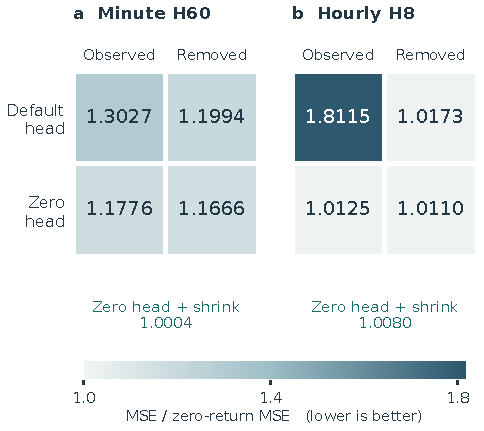
\includegraphics[width=\columnwidth]{figures/return_factorial.pdf}
\caption{Initialization and anchor interventions in xPatch. Cells show endpoint MSE divided by zero-return MSE, averaged over seeds at each origin. The shared shading measures excess error; 1 is the reference. The separate values below the grids add inner-stop shrinkage to the zero-head, observed-anchor cell.}\label{fig:factorial}
\end{figure}

Removing the anchor is especially consequential for default hourly H8: the normalized error falls from 1.8115 to 1.0173. Combining anchor removal with initialization yields only a small further change. The positive factorial interaction in trained loss is supported under both block lengths, indicating overlapping benefits rather than two additive gains. This comparison implicates the implemented anchor and initialization routes, while leaving their economic interpretation open.

Here the interaction is \(L_{\rm both}-L_{\rm init}-L_{\rm no\ anchor}+L_{\rm default}\), using paired losses from the four trained cells. A positive value means that adding the two separate error reductions overstates the reduction obtained together. The matrix makes this visible: the hourly default with an observed anchor is far from the other three cells. At minute H60, all four trained errors remain appreciably above the reference, even after the changes. We therefore retain the task distinction when interpreting the same intervention.

The hourly price result is larger in magnitude (Fig.~\ref{fig:cap}). Default LSTM error falls from 769.51 to 269.68 USD\(^2\) with the higher cap; default xPatch falls from 6,494.47 to 4,641.93. Current-price initialization reaches 1.9039 and 1.9053 within twenty epochs. Persistence is 1.8985. More updates help the default, but they do not reproduce the initialization result within the tested budget. Both initialized networks remain slightly worse than persistence.

The continuation also clarifies what the experiment measures. Early stopping prevents further updates in thirteen fits, so raising the cap does not assign sixty epochs to every model. For the cap-bound fits it permits further optimization along the original trajectory. The result concerns this optimizer and stopping procedure at the stated limits. It cannot rank the architectures after unrestricted tuning, nor establish how long the default would need to reach persistence.

\begin{figure}[t]
\centering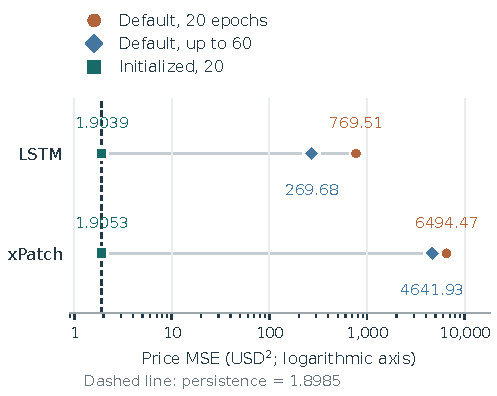
\includegraphics[width=\columnwidth]{figures/cap_comparison.pdf}
\caption{Hourly-H1 price error. Connected points compare the continued default fits with current-price initialization; positions follow a logarithmic MSE axis. Direct labels retain the small difference between initialization and persistence. The sixty-epoch arm continues the original checkpoints under the same stopping rule.}\label{fig:cap}
\end{figure}

For a return or price-change forecast \(p\),
\[
E[(y-p)^2]=E[y^2]+E[p^2]-2E[yp].
\]
A model can therefore lower error by reducing forecast energy \(E[p^2]\), without gaining enough alignment \(E[yp]\) to beat a zero change. Inner-stop shrinkage brings the two designated return forecasts close to zero, but their final gains are still \(-0.038\)\% and \(-0.795\)\%. This accounts for the apparent discrepancy between a large improvement over the default and little useful departure from the reference.

\subsection{Long-scale gains depend on the comparison}

Table~\ref{tab:tasks} retains every task under the same initialization-and-shrinkage rule. Intraday errors cluster near, or above, persistence/zero; the conspicuous positive results are annual. Their three-seed price and return gains are 33.731\% and 38.105\% over 47 overlapping origins. Four price folds and all five return folds improve. The shrunk unconditional mean also gains 23.249\% and 32.804\%.

\begin{table}[t]
\centering\small
\caption{Endpoint-MSE improvement of the fixed xPatch recipe over persistence/zero. P/R gives price/return seed counts. Long-scale entries use the later three-seed follow-up; the recipe is not selected separately for each task.}\label{tab:tasks}
\setlength{\tabcolsep}{4pt}
\begin{tabular}{lrrc}\toprule
Task & Price & Return & Seeds P/R\\\midrule
Annual H12 & +33.731\% & +38.105\% & 3/3\\
Quarterly H3 & +1.226\% & +0.698\% & 3/3\\
Monthly H21 & +0.063\% & +0.741\% & 3/3\\
Hourly H1 & $-0.209$\% & $-0.796$\% & 3/1\\
Hourly H4 & $-0.061$\% & $-0.517$\% & 1/1\\
Hourly H8 & $-1.636$\% & $-0.795$\% & 1/3\\
Minute H5 & $-0.011$\% & $-0.010$\% & 1/1\\
Minute H15 & $-0.035$\% & +0.003\% & 1/1\\
Minute H30 & $-0.138$\% & $-0.339$\% & 1/1\\
Minute H60 & $-0.066$\% & $-0.038$\% & 1/3\\\bottomrule
\end{tabular}
\end{table}

Figure~\ref{fig:annual} displays the paired annual intervals against each reference. The intervals against persistence/zero lie above zero, whereas both block lengths include zero against the shrunk mean. The gain percentages have different denominators: the repair's 33.731\% price gain over persistence is not a 33.731\% gain over the mean. On the original four-path nonoverlapping subset, repair gains are 17.585\%/7.470\% for price/return, compared with 48.349\%/51.317\% for the mean. This dependent sensitivity check reverses the pooled ranking and leaves very little event diversity.

Successive annual origins share most of their twelve-month target windows. A prolonged market movement can therefore influence many errors in the pooled score. Grouped resampling preserves some of this dependence, but its intervals still describe the available history. The four-path subset removes target overlap at the cost of almost all sample size. Agreement across seeds can coexist with either problem because the seeds change the fit, not the realized target paths.

\begin{figure}[t]
\centering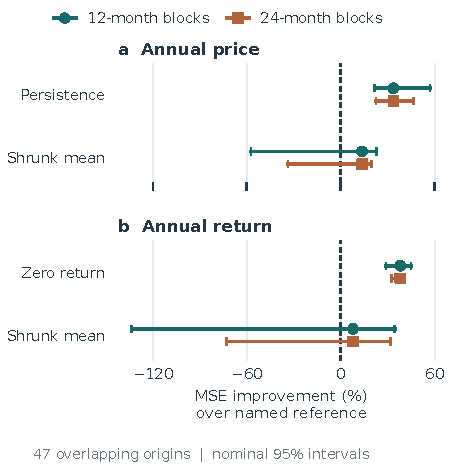
\includegraphics[width=\columnwidth]{figures/annual_intervals.pdf}
\caption{Annual gains with stronger references. Dots/squares show the same repaired forecast; horizontal lines are saved paired nominal 95\% intervals at two block lengths. Every row uses its named reference as denominator. Intervals are shown in full, including wide negative bounds against the shrunk mean.}\label{fig:annual}
\end{figure}

Quarterly-H3 returns offer a narrower contrast. The repair gains 0.698\% over zero and beats the shrunk mean with nominal intervals [0.15\%, 1.18\%] and [0.18\%, 1.04\%]. All pooled seed gains are positive, but only one of five fold means improves over zero. The raw mean and selected Ridge gain 1.784\% and 20.948\%, respectively, and both have lower pooled error than the repair. The comparison uses 52 overlapping origins.

Fixed-weight annual history substitutions provide another caution. Replacing histories with fit-mean histories changes price/return gains to 2.814\%/14.826\%; flat histories produce 49.756\%/49.176\%. The weights and calibration are unchanged. Such inputs may be out of distribution, so this is a sensitivity probe rather than an improved trained model. It does show that the annual result cannot be attributed confidently to useful reading of the observed trajectory (Supplement S1--S8).

\subsection{One split changes the monthly reference}\label{sec:split}

Apple announced a four-for-one split on July 30, 2020, with split-adjusted trading effective August 31 \cite{r19}. Persistence ignores that public announcement even when a nominal-price target crosses the effective date. We therefore calculate a separate announcement-based reference after examining the event. Its conservative eligibility boundary is August 1, 00:00 New York, supported by the as-filed 10-Q and SEC metadata. Figure~\ref{fig:split} separates announcement, information eligibility and trading effect.

For eligible origins before August 31 whose future coordinate reaches that date, the reference predicts \(P_t/4\) or \(-\log 4\). All other coordinates retain persistence/zero. The nominal targets, model predictions and original assessment origins stay fixed. Of 1,970 monthly-H21 origins, 21 eligible paths cross the event, affecting 231 path coordinates per target. They share one corporate action.

The nominal target records a change in the quoted price per share. Across a split, that change differs from an investor's wealth return because the share count also changes. A large split-crossing log-return error is thus not evidence of failing to predict an equivalent loss of wealth. Retaining the original target lets us isolate the effect of reference information. A fully adjusted-price or total-return study would define another target and would require a separate comparison.

\begin{figure}[t]
\centering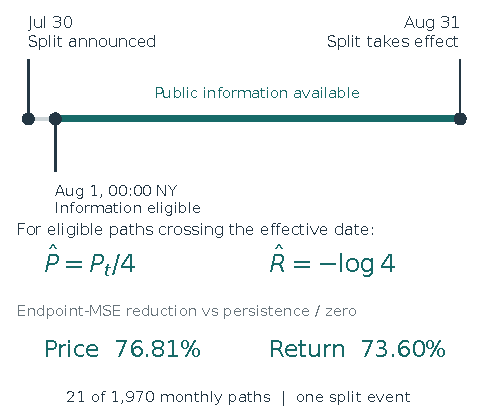
\includegraphics[width=\columnwidth]{figures/split_event.pdf}
\caption{The 2020 announced split changes the reference information. Calendar spacing is proportional; this is an event timeline, not a price trajectory. Reductions pool all monthly endpoint errors under the original targets. The 21 eligible paths are overlapping views of one event.}\label{fig:split}
\end{figure}

The new reference reduces monthly price and return endpoint MSE by 76.809\% and 73.597\%. Re-expressing saved repaired-model losses against it changes the model's gains from 0.063\%/0.741\% to \(-330.938\)\%/\(-275.931\)\%. No assessed annual or quarterly path crosses this event. This result identifies a material omission in the close-only reference. Because the reference receives additional public information, the calculation does not compare architectures under an equal information set, nor does it test a model trained with the announcement (S32).

\subsection{A restriction inside the short-horizon trend branch}

Source inspection identifies a separate deterministic restriction in xPatch. At native H2/H3, a trend-branch LayerNorm receives a single coordinate \(u\). Its mean is \(u\), its variance is zero, and
\[
\operatorname{LN}(u)=\gamma\frac{u-u}{\sqrt{0+\epsilon}}+\beta=\beta,
\qquad \frac{\partial\operatorname{LN}(u)}{\partial u}=0.
\]
That branch output is independent of its trend input. The H1 adapter calls native H2, so hourly-H1 and quarterly-H3 price/return tasks are affected. Eight synthetic checks confirm the restriction. Seasonal and anchor routes remain active: this is not a constant-output claim for the full model, and it does not explain the H60/H8 errors (S22).

\section{Additional experiments}\label{sec:followups}

\subsection{Attempts to improve the conditional mean}

The diagnostics motivated further tests of normalization, compressed history, fixed expert combinations, genuine horizon sharing, session representations and recurrent-state routing. None met its specified predictive or continuation rule. Price--volume, close-location and delayed-SPY inputs were also screened; the volume hypotheses draw on \cite{r17,r18}. These additions did not establish a stable gain over the controls. Calendar, event-support, level and artificial-signal probes helped delimit particular explanations, while one local-gradient route remained numerically unresolved. Their protocols, exclusions and results are retained in S7 and S11--S38. We do not use a successful isolated fold from these attempts to replace the full comparison.

\subsection{A small distributional forecasting screen}

A separate two-fold screen asks whether uncertainty is easier to predict than the return mean. Location stays at zero. All arms use Student-t densities with five degrees of freedom and scale \(s^2=3v/5\), where \(v\) is the predicted variance. B0 has a constant scale. B1 uses EWMA variance with decay 0.94 and fit-prefix calibration \cite{r20}. B2 regresses log variance on short, daily and twenty-session summaries, motivated by heterogeneous volatility horizons \cite{r21}. This HAR-type control is not a replication of daily HAR-RV. Candidate C adds sine/cosine clock coordinates and the calendar-known number of session boundaries.

The fitting rule and support mask are set before scoring. Longer history removes unsupported early fit origins, but no outer origins. Six recipes, including two ablations, give 24 positions and 22 unique fits; two minute positions reuse C because their gap count is zero. Table~\ref{tab:probability} reports paired NLL differences in the same return units. A positive difference favors C; density NLL itself can be negative.

\begin{table}[t]
\centering\small
\caption{Two-fold distributional screen. \(\Delta\)NLL is reference minus C in nat/origin. Coverage is the observed share inside C's central intervals.}\label{tab:probability}
\setlength{\tabcolsep}{4pt}
\begin{tabular}{lrr}\toprule
Quantity & Minute H60 & Hourly H8\\\midrule
Evaluation origins & 151,440 & 2,718\\
\(\Delta\)NLL vs B0 & +0.11850 & +0.06234\\
\(\Delta\)NLL vs B1 & +0.02513 & $-0.00715$\\
\(\Delta\)NLL vs B2 & +0.00217 & +0.00930\\
50\% coverage & 46.56\% & 40.91\%\\
90\% coverage & 89.35\% & 84.77\%\\
Task screen & Pass & Fail\\\bottomrule
\end{tabular}
\end{table}

C passes the minute screen but trails hourly EWMA by 0.00715 nat/origin; its hourly 90\% interval covers only 84.77\%. The rule requires both tasks to pass, so the screen stops without the other three folds. B1 and B2 both beat B0 in pooled NLL on each task, although hourly B1 does not win in every fold. The result suggests conditional-scale information but establishes neither a cross-frequency improvement nor a conditional-mean gain. The separate addendum retains CRPS, all scores and the stopping decision.

\section{Discussion and conclusion}\label{sec:discussion}

The hourly price experiment shows why initialization belongs in a model comparison. Under the tested caps, a current-price initial function does more to reduce error than tripling the default training allowance. The return interventions show the limit of that repair: large reductions relative to a weak default leave the forecast near zero. A useful architecture claim would need to survive the second comparison as well as the first.

Long-scale results call for a different explanation. Annual gains over persistence/zero coexist with inconclusive comparisons against an unconditional mean, few nonoverlapping outcomes and strong sensitivity to input substitutions. At the monthly scale, accounting for an announced split changes the reference error dramatically. A ranking across these tasks consequently mixes optimization behavior, reference information and market history. Reporting only its winners would conceal the most informative parts of the study.

There are substantial limits to inference. Assessment periods were inspected during development; subsequent screens and nominal intervals cannot supply an unseen market test. Additional seeds measure training variability rather than add market episodes. The protected 2026Q3 period remains unscored, and a single quarter could not confirm annual H12 targets. Finalized vendor bars, assumed completion times, revisions, excluded dividends and the concentration of split-crossing errors further restrict interpretation. This is a single-stock forecast study without a strategy, transaction-cost model or profitability evaluation.

The supported result is a measured implementation effect and an account of why some apparent gains weaken under better controls. Zero-head initialization, scalar shrinkage and split adjustments are established ideas; we do not present them as a new forecasting architecture. A subsequent method study would need to fix its candidate before evaluating fresh periods, retain unconditional and information-matched controls, and test more equities with their own corporate actions and session clocks. The present experiments provide the comparisons needed to design that test; they have not yet demonstrated the stable predictive gain it would seek.

\section*{Data and code availability}

The accompanying package contains editable LaTeX, plotting aggregates, vector figures, the 41-page supplement and a separate probability-screen addendum. The reproduction guide identifies the external data, checkpoints and computation records required for full experimental replication. The supplied figures can be regenerated without those dependencies.

\begin{thebibliography}{99}

\small\setlength{\itemsep}{0pt}\setlength{\parskip}{0pt}

\bibitem{r1} Stitsyuk, A., and Choi, J. ``xPatch: Dual-Stream Time Series Forecasting with Exponential Seasonal-Trend Decomposition.'' \emph{Proceedings of the AAAI Conference on Artificial Intelligence}, 39(19), 20601--20609, 2025. \url{https://doi.org/10.1609/aaai.v39i19.34270}

\bibitem{r2} Nie, Y., Nguyen, N. H., Sinthong, P., and Kalagnanam, J. \emph{A Time Series is Worth 64 Words: Long-term Forecasting with Transformers}. arXiv:2211.14730, version 2. \url{https://arxiv.org/abs/2211.14730v2}

\bibitem{r3} Lim, B., Arik, S. O., Loeff, N., and Pfister, T. \emph{Temporal Fusion Transformers for Interpretable Multi-horizon Time Series Forecasting}. arXiv:1912.09363, version 3. \url{https://arxiv.org/abs/1912.09363v3}

\bibitem{r4} Kumbure, M. M., Lohrmann, C., Luukka, P., and Porras, J. ``Machine Learning Techniques and Data for Stock Market Forecasting: A Literature Review.'' \emph{Expert Systems with Applications}, 197, 116659, 2022. \url{https://doi.org/10.1016/j.eswa.2022.116659}

\bibitem{r5} Zhang, Z., Zohren, S., and Roberts, S. \emph{DeepLOB: Deep Convolutional Neural Networks for Limit Order Books}. arXiv:1808.03668, version 6. \url{https://arxiv.org/abs/1808.03668v6}

\bibitem{r6} Ballarin, G., Capra, J., and Dellaportas, P. \emph{Multi-Horizon Echo State Network Prediction of Intraday Stock Returns}. arXiv:2504.19623, version 1, 2025. \url{https://arxiv.org/abs/2504.19623v1}

\bibitem{r7} Shi, Y., Fu, Z., Chen, S., Zhao, B., Xu, W., Zhang, C., and Li, J. \emph{Kronos: A Foundation Model for the Language of Financial Markets}. arXiv:2508.02739, version 1, 2025. \url{https://arxiv.org/abs/2508.02739v1}

\bibitem{r8} Kamalov, F., Gurrib, I., and Rajab, K. D. ``Financial Forecasting with Machine Learning: Price Vs Return.'' \emph{Journal of Computer Science}, 17(3), 251--264, 2021. \url{https://doi.org/10.3844/jcssp.2021.251.264}

\bibitem{r9} Mattera, R., Athanasopoulos, G., and Hyndman, R. J. ``Improving Out-of-Sample Forecasts of Stock Price Indexes with Forecast Reconciliation and Clustering.'' \emph{Quantitative Finance}, 24(11), 1641--1667, 2024. \url{https://doi.org/10.1080/14697688.2024.2412687}. Author-hosted manuscript consulted: \url{https://robjhyndman.com/papers/dow_hts.pdf}.

\bibitem{r10} Bergmeir, C., and Benítez, J. M. ``On the Use of Cross-Validation for Time Series Predictor Evaluation.'' \emph{Information Sciences}, 191, 192--213, 2012. \url{https://doi.org/10.1016/j.ins.2011.12.028}

\bibitem{r11} Künsch, H. R. ``The Jackknife and the Bootstrap for General Stationary Observations.'' \emph{The Annals of Statistics}, 17(3), 1217--1241, 1989. \url{https://doi.org/10.1214/aos/1176347265}

\bibitem{r12} Alpaca. \emph{Market Data FAQ: How are bars aggregated?} \url{https://docs.alpaca.markets/us/docs/market-data-faq}

\bibitem{r13} Bai, S., Kolter, J. Z., and Koltun, V. \emph{An Empirical Evaluation of Generic Convolutional and Recurrent Networks for Sequence Modeling}. arXiv:1803.01271, 2018. \url{https://arxiv.org/abs/1803.01271}

\bibitem{r14} Bates, J. M., and Granger, C. W. J. ``The Combination of Forecasts.'' \emph{Operational Research Quarterly}, 20(4), 451--468, 1969. \url{https://doi.org/10.1057/jors.1969.103}

\bibitem{r15} Jacobs, R. A., Jordan, M. I., Nowlan, S. J., and Hinton, G. E. ``Adaptive Mixtures of Local Experts.'' \emph{Neural Computation}, 3(1), 79--87, 1991. \url{https://doi.org/10.1162/neco.1991.3.1.79}

\bibitem{r16} Campbell, J. Y., and Thompson, S. B. ``Predicting Excess Stock Returns Out of Sample: Can Anything Beat the Historical Average?'' \emph{The Review of Financial Studies}, 21(4), 1509--1531, 2008. \url{https://doi.org/10.1093/rfs/hhm055}

\bibitem{r17} Campbell, J. Y., Grossman, S. J., and Wang, J. ``Trading Volume and Serial Correlation in Stock Returns.'' \emph{The Quarterly Journal of Economics}, 108(4), 1993. \url{https://doi.org/10.2307/2118454}

\bibitem{r18} Llorente, G., Michaely, R., Saar, G., and Wang, J. ``Dynamic Volume-Return Relation of Individual Stocks.'' \emph{The Review of Financial Studies}, 15(4), 1005--1047, 2002. \url{https://doi.org/10.1093/rfs/15.4.1005}

\bibitem{r19} Apple Inc.~\emph{Form 10-Q for the quarter ended June 27, 2020}, pp.~18 and 32; SEC accession 0000320193-20-000062, filed July 31, 2020. \url{https://s2.q4cdn.com/470004039/files/doc_financials/2020/q3/_10-Q-Q3-2020-(As-Filed).pdf}

\bibitem{r20} J.P. Morgan/Reuters. \emph{RiskMetrics---Technical Document}, 4th ed., 1996. \url{https://www.msci.com/documents/10199/5915b101-4206-4ba0-aee2-3449d5c7e95a}

\bibitem{r21} Corsi, F. ``A Simple Approximate Long-Memory Model of Realized Volatility.'' \emph{Journal of Financial Econometrics}, 7(2), 174--196, 2009. \url{https://doi.org/10.1093/jjfinec/nbp001}

\end{thebibliography}

\end{document}
